% !TeX spellcheck = es
\documentclass{report}
\usepackage[utf8]{inputenc}

% Títulos automáticos en español
\usepackage[spanish]{babel}

% Soporte para buenas urls e hipervínculos entre secciones
\usepackage{hyperref}

% Citas y referencias en formato APA
% Si quiere las citas y referencias en IEEE comente esta línea
\usepackage{apacite}

% Imágenes y figuras
\usepackage{graphicx}

% Código fuente con números de línea
\usepackage{listings}
% Puede cambiar el lenguaje de código fuente
% https://www.overleaf.com/learn/latex/code_listing#Supported_languages
\usepackage{multirow}


\lstset{
    language=C,
    basicstyle=\footnotesize,
    numbers=left,
    stepnumber=1,
    showstringspaces=false,
    tabsize=1,
    breaklines=true,
    breakatwhitespace=false,
}


\def \unidad{Escuela de Ingeniería en Computación}
\def \programa{Ingeniería en Computación}
\def \curso{IC6600 - Principios de Sistemas Operativos}
\def \titulo{Proyecto 1}
\def \subtitulo {Codificación de Huffman}
\def \autores{
    Gerald Calderón\\
    Correo electrónico\\
    Carnet\\
    
    \vspace{0.5cm}
    
    Óscar Obando\\
    osobando@estudiantec.cr\\
    2023091684
    
    \vspace{0.5cm}
    
    Samuel Zúñiga\\
    Correo electrónico\\
    Carnet
}
\def \fecha{Septiembre 2025}
\def \lugar{
    San José, 
    Costa Rica
}

% Inicia el documento 
\begin{document}

% Inserta la portada del documento
\begin{titlepage}
    \begin{center}
        \vspace*{1cm}
        
        
\includegraphics[width=0.8\linewidth]{figuras/logo_tec.jpg}\\
        \LARGE
        \unidad\\
        \programa\\
        \curso
        
        \vspace{1cm}
        
        \Huge
        \textbf{\titulo}
            
        \vspace{0.5cm}
        \LARGE
        \subtitulo
            
        \vspace{1.5cm}
        
        \large    
        \autores
            
        \vfill
        
        \lugar\\
        \fecha
        
    \end{center}
\end{titlepage}

\tableofcontents

\chapter{Introducción}\label{intro}

Para este proyecto se implementó un compresor (y decompresor) de archivos de texto utilizando el algoritmo de Huffman.
Este toma un directorio con archivos de texto y los comprime en un solo archivo en binario, al descomprimir, se restaura el directorio y los archivos dentro de este.
Este sistema consiste en dos partes principales,  el programa que comprime y el programa que descomprime.
Ambos ofrecen tres modos de ejecución: serial, concurrente y paralelo.

\section {Proyecto Gutenberg}

Este proyecto fue probado con los top 100 libros de los últimos 30 días del proyecto Gutenberg.
Este proyecto, fundado por Michael  Hart, consiste en una colección de libros electrónicos gratuitos, que son versiones digitalizadas de libros que existen en físicamente \cite{ref0}.
Esta colección ofrece múltiples formatos para descargar y leer libros, entre estos texto con formato UTF-8, el cual fue usado para este proyecto.

\section{Algoritmo de Huffman}

El algoritmo de Huffman es un algoritmo de compresión de texto, creado por David Huffman en 1952 \cite{ref2}.
Este fue creado ya que su profesor ofreció a sus estudiantes dos opciones: hacer el examen final, o escribir un paper sobre cómo encontrar el código óptimo para todos los símbolo en un texto.
Lo que su profesor no explicó,  es que este problema era un problema abierto y que él mismo estaba trabajando en él.
Luego de pensar por mucho tiempo,  Huffman inventó un algoritmo que utiliza un árbol binario para encontrear dichos códigos óptimos. 


Lo primero para entender este algoritmo es entender que las computadoras guardan información de texto en formatos como ASCII o UNICODE, cada símbolo dentro de estos estándares tienen un código único que permite a la computadora diferenciarlos entre sí \cite{ref3}.
El problema con estos estándares es que se le asigna la misma cantidad de bytes a todos los símbolos,  esto significa que un símbolo muy común, tiene el mismo tamaño que uno poco común.
Idealmente los símbolos más comúnes deberían tener un tamaño más pequeño. 

El algoritmo de Huffman busca compactar el texto, encontrando los símbolos más comunes en un texto y mapeando cada uno a un código nuevo \cite{ref3}.
Para esto, se cuenta la cantidad de veces que aparece cada símbolo en el texto y a cada uno se les asigna un código en binario, entre más común el símbolo más corto su código.
Se arma un arbol binario en dónde cada nodo interno tiene la posibilidad de conectarse con un hijo por medio de un 1 o un 0, al recorrer un camino específico del arbol desde la raíz hasta una hoja, se forma el código que representa un símbolo del texto. 



\section {Algoritmos de compresión con y sin pérdida}

El algoritmo de Huffman es un algoritmo de compresión sin pérdida, esto significa que al comprimirse no se pierde contenido alguno del archivo \cite{ref4}.
La compresión sin pérdida remueve metafata innecesaria en el archivo, que luego puede ser reconstruida para su uso.
Esto es útil cuando se tiene archivos que paran de terne sentido para el usuario si se pierde su contenido, como archivos de texto.
Pero este no es el único tipo de algoritmos de compresión, ya que, existen los algoritmos de compresión con pérdida.

Como su nombre lo explica, un algoritmo de compresión con pérdida, es un algoritmo que comprime el tamaño del archivo borrando información permanentemente \cite{ref4}.
Este tipo de información puede ser útil cuando el archivo sigue teniendo sentido para el usuario incluso si se perdió parte del contenido binario.
Un ejemplo de esto es una imagen,  al comprimirse es posible que esta sea un poco más borrosa que antes, pero esta sigue teniendo sentido y en el mejor caso, la diferencia no puede ser vista por el ojo humano.


\section{Paralelismo y concurrencia}

Como dicho anteriormente, para este proyecto se solicitó crear 3 modos de ejecución para cada comprimir y descomprimir los archivos. 
Serial es el modo de ejecución más fácil de estos tres, y este modo de ejecución es cuando una tarea completa es hecha en un solo procesador, sin separar la ejecución de las subtareas.
Mientras que su facilidad de uso da muchas ventajas, los siguientes dos modos de ejecución proveen ventajas como tener un mejor tiempo de ejecución cuando son utilizados correctamente.

Concurrencia es cuando se está trabajando una tarea, y se divide esta en subtareas que son independientes las unas de las otras, pero no necesariamente se corren al mismo tiempo.
Cada tarea concurrente, toma turnos en el mismo procesador \cite{ref1}.
Esto es útil ya que es posible que cada tarea no solo necesite tiempo del procesador, si no que es posible que necesite otros servicios, como I/O, por lo que hace que se administre mejor el tiempo que utiliza cada hilo en cada servicio que necesita. 
Esta necesita un cambio de contexto cada vez que el procesador va a cambiar de hilo. 

Paralelismo, es cuando se ejecutan varias subtareas independientes al mismo tiempo, en distintos procesadores \cite{ref1}. 
Esto permite que un solo programa pueda aprovechar más su uso del los recursos de la computadora, teniendo varios programas hijo que se encargan de subtareas.
Este no necesita cambiar de contexto, ya que cada sub tarea es ejecutada en un programa individual, por lo que no es necesario cambiar el contexto. 

La gran diferencia entre estos es que la concurrencia trata sobre manejar múltiples computaciones manejando el uso del CPU, mientras que el paralelismo corre múltiples computaciones al mismo tiempo \cite{ref1}.
Se puede notar que la concurrencia no es realmente que los hilos corren al mismo tiempo, si no que se intercalan los usos del CPU, dándo la ilusión de que corren al mismo tiempo. Además, por su naturaleza, la concurrencia puede correr en un solo procesador, pero el paralelismo necesita uno o más obligatoriamente.
Hay una división bastante clara entre estos dos, ya que el objetivo de la concurrencia es mejorar la eficiencia aprovechando el tiempo en dónde una parte del programa está esperando por I/O, mientras que la paralelización busca mejorar la eficiencia del programa haciendo múltiples tareas al mismo tiempo. 



\chapter {Desarrollo}

\section {Función fork() y biblioteca pthread}

\subsection {Función fork() en C}

La función \texttt{fork()} en el lenguaje de programación C es usada para duplicar el proceso el cuál la llama \cite{ref5}.
Cuando un proceso se duplica se obtienen dos procesos, el proceso padre y el proceso hijo, el cuál es la dúplica del padre.
La función \texttt{fork()} no toma ningún parámetro y devuelve un número entero: si este número es negativo, significa que no se logró crear el proceso hijo; si este número es 0, indica que el proceso el cuál leyó el valor es el proceso hijo; finalmente, si este valor es positivo, indica que el proceso es el padre, más específicamente, este valor corresponde a el ID del hijo creado. 
Además, si el proceso padre se cierra inesperadamente, el proceso hijo también es matado.

Una vez se crea el proceso hijo, es posible que se quiera que este solo corra una parte específica del código.
Para manejar esto se utilizan las funciones \texttt{exit()} y \texttt{wait()}.
La función \texttt{exit()} debe ser llamada desde un proceso hijo, una vez esto ocurre, el proceso hijo termina inmediatamente; además, esta función toma un número entero como parámetro, este se usa para revisar el estado de salida del hijo.
La función \texttt{wait()} es usada en el proceso padre esta hace que el padre espera a que el hijo termine antes de seguir con su ejecución, esta función toma como parámetro una referencia a un entero, una vez el hijo termina, se agrega el estado de salida del hijo a esta referencia, si no se quiere recibir el estado de salida simplemente se puede usar \texttt{wait(NULL)}.

\subsection {Biblioteca pthread en C}


\section {Estrategias para paralelizar los programas}


\section{Desarrollo}

\subsection{Descripción del proyecto}
El proyecto presentado trata sobre la implementación de un programa de compresión y descompresión de directos de archivos de texto plano. Está diseñado específicamente para la distribución de Debian, pero puede ser ejecutado en otras distribuciones de Linux que compartan las mismas características. La diferencia rige en el archivo de instalación de paquetes necesarios como gcc y make. Sin embargo, estos pueden ser instalados manualmente por el usuario que desee utilizar el programa.

La implementación de este algoritmo se hace en base a los presentado en el capítulo 16 del libro Algoritmos a fondo \cite{book_huffman}. Para realizar las labores de compresión se realiza la utilización del algoritmo de Huffman, éste consiste en tomar las frecuencias de cada conjunto de caracteres presentados en el archivo y crear una lista que los ordene de manera ascendente. Posteriormente se crea el árbol de Huffman. Para formar el árbol se realiza la eliminación de los dos primeros nodos de la lista y se agregan a un nuevo nodo que contenga la suma de sus frecuencias. El nodo con menor frecuencia se coloca a la derecha (el primero) y el de mayor frecuencia a la izquierda (el segundo). Luego este nodo se inserta de nuevo a la lista siguiendo el ordenamiento por frecuencia, y así se realiza sucesivamente hasta tener un solo elemento que sería la raíz del árbol.

Una vez creado el árbol se visitan recursivamente los hijos de la raíz para formar el diccionario del código en binario para cada carácter leído de los archivos. Este diccionario se forma concatenando un 0 al código si es que está hacía la derecha del nodo actual o un 1 si está a la izquierda, esto se realiza hasta llegar a un nodo hoja que representaría el carácter buscado.

Con el diccionario formado la compresión del archivo se reduce simplemente a ir reemplazando cada carácter por su equivalente en el archivo de salida objetivo. Para facilitar la descompresión se agrega al inicio del archivo el diccionario formado seguido por el nombre del primer archivo comprimido y la cantidad de bits que este representa. De esta manera, cuando se va a descomprimir se extrae primero el árbol, luego el nombre del archivo junto con su tamaño en bits y posteriormente se realiza la descompresión de dicho archivo, cuando la cantidad de bits reemplazados llegan al total que poseía dicho archivo se estaría cerrando y guardando para procesar el siguiente. Este proceso se realiza repetidamente hasta que no hayan archivos o bits por leer.

\begin{figure}[h]
    \centering
    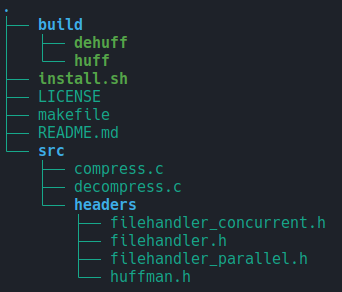
\includegraphics[width=0.8\linewidth]{figuras/estructura.png}
    \caption{Ilustración de la estructura del programa}
    \label{fig:estructura}
\end{figure}

\subsection{Instrucciones}
\subsubsection{Cómo instalar el programa}
\begin{enumerate}
  \item Descargue el código fuente del programa. Puede hacerlo de las dos siguientes formas:
    \begin{itemize}
      \item Dirigirse al repositorio de GitHub mediante su navegador a través del siguiente link: \url{https://github.com/Andres2950/SO\_Huffman.git}
      \item Instalarlo directamente con el comando \\
    \texttt{wget \url{https://github.com/Andres2950/SO\_Huffman/archive/refs/heads/main.zip}}
    \end{itemize}
  \item Descomprima el archivo .zip descargado utilizando el comando \texttt{unzip}.
  \item Al extraer el archivo podrá observar la estructura de organización similar a la figura \ref{fig:estructura}.
\item Ejecute el archivo \texttt{install.sh}, asegúrese de qué tenga permisos de ejecución, puede utilizar el comando \texttt{chmod +x install.sh} en caso de que no los posea y luego ejecute de la siguiente forma \texttt{./install.sh}. \\
  Este archivo se hará cargo de la instalación del compilador \textit{gcc} necesario para compilar el código fuente. Además hará la instalación del paquete \textit{make} para la ejecución de archivos makefile, dicho archivo posee las instrucciones de compilación de \textit{gcc} para resolver todas las dependencias que se encuentran en el directorio \textit{src/headers}.  
\item Note que la instalación de dichos paquetes requiere permisos de usuarios root, al ejecutar el archivo \texttt{install.sh} este se volverá a ejecutar con dichos permisos, para esto solicitará la contraseña del usuario root para tener dichos permisos de ejecución (la contraseña es totalmente invisible para el programa) y así poder descargar los paquetes. Mostrará un mensaje como el de la figura N y esperará la entrada correcta.
\item La compilación de los archivos se realiza sin permisos root.
\item Además, el \texttt{install.sh} hará una copia de los binarios \texttt{huff} y \texttt{dehuff} en el directorio \textit{/usr/bin} de la máquina para poner ser accedidos desde cualquier lugar y utilizado en múltiples directorios sin necesidad de mover los archivos a comprimir o descomprimir a una carpeta en particular.

\end{enumerate}

\subsubsection{Cómo utilizar el programa}
Una vez terminado el procedimiento de instalar el programa puede utilizar el comando huff para comprimir archivos. Dicho comando posee una serie de parámetros para sus distintos modos de ejecución. A continuación se detallan cada uno.

\begin{figure}[h]
    \centering
    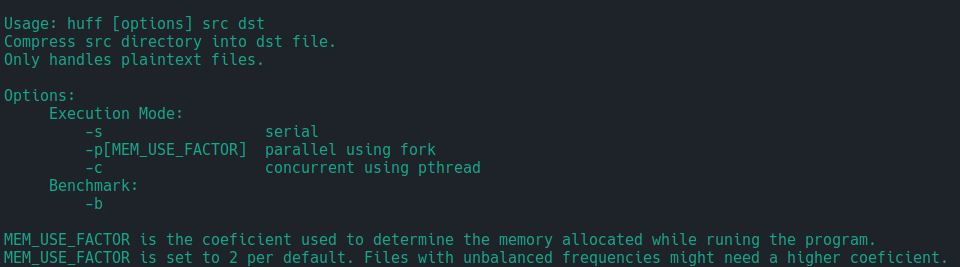
\includegraphics[width=0.8\linewidth]{figuras/huff_ayuda.png}
    \caption{Ilustración del menú de ayuda del comando huff -h}
    \label{fig:huffayuda}
\end{figure}

\begin{itemize}
  \item \textbf{huff -h}\\ \hspace{2cm}
    Provee una guía de los parámetros requeridos por el programa y su orden de entrada (Véase figura \ref{fig:huffayuda}).
  \item \textbf{huff [Opción] src dst} o \textbf{dehuff [Opción] src dst}\\
src es el directorio objetivo a ser comprimido/descomprimido\\
dst es el archivo de destino
  \item \textbf{Opciones} 
    \begin{itemize}
      \item \textbf{-s} modo de ejecución serial.
      \item \textbf{-p} modo de ejecución paralela usando fork.
      \item \textbf{-c} modo de ejecución concurrente usando pthread
      \item \textbf{-b} modo de Benchmark para comparar los tiempos de ejecuión entre los anteriores modos.
    \end{itemize}
\end{itemize}





\section{Discusión}
\subsection{Resultados de las pruebas}
\subsubsection{Metodología de las pruebas}

Las pruebas que se realizaron tenían el objetivo de obtener el tiempo de ejecución del programa o una parte de este. Para lograr esto se decidió tomar marcas de tiempo en el código al inicio y al final de la parte que se quería probar. Se utilizó el header time.h tomar los tiempos. El tiempo de ejecución  se imprime en pantalla como la diferencia entre las dos marcas de tiempo.

Se realizaron pruebas en distintas partes de los programas y cada prueba se realizó en las 3 implementaciones diferentes. En total se probó el sistema completo del compresor y sus subsistemas de lectura y compresión; y el sistema completo del descompresor y su subsistema de descompresión y escritura.

Cada prueba se ejecutó 50 veces de forma independiente. La tabla de resultados contiene el promedio de las 50 pruebas.

\subsubsection{Tabla de resultados}

\begin{center}
	\begin{tabular}{|c|c|c|c|}		
		
\hline
\multicolumn{4}{|c|}{Tiempo de Ejecución (milisegundos)} \\
\hline
 Subsistema& \multicolumn{3}{|c|}{Versión} \\
 \hline
 & Serial & Concurrente & Paralelo\\
 \hline
huff(completo) & 5360& 2226 & 2036\\
 \hline
huff(lectura) &  36 & 25 & 19\\
 \hline
 huff(compresión) &  5168 & 1957 & 1681\\
 \hline
 dehuff(completo) & 5189 & 2092 & 1855\\
 \hline
 dehuff(descompresión y escritura) & 5146 & 1968 & 1629\\
 \hline
 
	\end{tabular}
\end{center}

\subsection{Análisis de aceleración}

\subsubsection{Metodología de Análisis}

Gene Amdahl (1922–2015) fue un informático especializado en arquitectura de hardware. Su contribución más conocida a la informática es su ley homónima, propuesta en 1967. 

La ley de Amdahl modela cuánto puede mejorarse el rendimiento del sistema al paralelizar el código. Muestra que, incluso con una potencia de cálculo infinita, las partes secuenciales limitan la aceleración. Esta ley ayuda a los desarrolladores a estimar las mejoras de rendimiento y a optimizar las secciones de código de alto impacto. La fórmula que representa la ley es la siguiente:



\begin{displaymath}	
	{T_{m} = {T_{a} \cdot \left((1 - F_{m}) + {F_{m} \over A_{m}}\right)}}
\end{displaymath}

Esta fórmula puede reescribirse para obtener la aceleración de un sistema completo luego de que se optimiza un subsistema. La formula sería la siguiente:

\begin{displaymath}	
	A = {1 \over (1 - F_{m}) + {F_{m} \over A_{m}}}	
\end{displaymath}
Donde:\\
$A$, es la aceleración o ganancia en velocidad conseguida en el sistema completo debido a la mejora de uno de sus subsistemas.\\
$A_{m}$, es el factor de mejora que se ha introducido en el subsistema mejorado.\\
$F_{m} $, es la fracción de tiempo que el sistema utiliza el subsistema mejorado.\\

La ley de Amdahl muestra que hay un limite en la aceleración posible que se puede obtener optimizando un programa. La siguiente re escritura de la fórmula nos da la aceleración máxima teórica para un sistema cuando N tiende a infinito.

	\begin{displaymath}	
		A = {2 \cdot \left 1 \over  S + {1-S \over N}}
	\end{displaymath}
Donde:\\
$A$, es la aceleración máxima conseguida en el sistema completo debido a la mejora de uno de sus subsistemas.\\
$S$, es la fracción del programa que es secuencial.\\
$N$,  el factor de mejora.\\

En las próximas secciones se realiza el cálculo par obtener la mejora de los programas de compresión y descompresión luego de haber sido optimizados mediante paralelización y concurrencia. Además se hace una discusión sobre las ganancias obtenidas a través de los diferentes métodos.

\subsubsection{Aceleración del compresor(huff)}

La ejecución del compresor se puede dividir en 3 fases: lectura, creación del árbol huffman, compresión y escritura. La etapa de lectura es donde se lee cada uno de los archivos del directorio fuente, esta etapa puede ser paralelizada.  La etapa de creación del  árbol huffman es donde se junta todo el texto para crear el diccionario con el código huffman, esta etapa no puede ser paralelizada. La etapa de compresión corresponde a la transformación de texto plano a codigo huffman de cada uno de los archivos, esta etapa puede ser paralelizada. La etapa de escritura es donde se escribe el código de cada archivo a un documento binario, esta etapa puede ser paralelizada pero se decidió no hacerlo.

La fracción del programa que abarca cada etapa sería: lectura(0.06), compresión(0.964), creación de árbol y escritura(0.02).  Lo que quiere decir que un 98\% del programa puede paralelizarse, esto implica que la aceleración máxima teórica del programa sería de 100.

La aceleración máxima que se logra obtener mediante el uso de hilos es de 2.341 y mediante el uso de fork es de 2.549. 

Ambas implementaciones mejoran drásticamente el tiempo de ejecución del programa. Ninguno de los dos se acercan al máximo teórico debido al overhead que tiene la paralelización, además el compresor cuenta con un cuello de botella en la etapa de creación del árbol huffman que se encuentra justo entre las dos etapas que se paralelizaron, lo que obliga el programa  a paralelizarse y serializarse dos veces.

Se puede observar que la implementación con paralela  fork es ligeramente más rápida que la  concurrente con hilos.

\subsubsection{Aceleración del descompresor(dehuff)}

La ejecución del descompresor se puede dividir en 2 fases: lectura del diccionario y reconstrucción del árbol, y descompresión y escritura. La primera etapa es donde se lee el inicio del archivo comprimido donde se encuentra el diccionario de códigos y se reconstruye el árbol en base a este, esta etapa no puede paralelizarse. La última etapa corresponde a la lectura del codigo de cada archivo, su descompresión y escritura, esta etapa puede ser paralelizada. 

La fracción del programa que abarca cada etapa sería: lectura de diccionario y reconstrucción de árbol (0.01), y descompresión y escritura(0.99).  Lo que quiere decir que un 99\% del programa puede paralelizarse, esto implica que la aceleración máxima teórica del programa sería de 200.

La aceleración máxima que se logra obtener mediante el uso de hilos es de 2.444 y mediante el uso de fork es de 2.727 

Ambas implementaciones mejoran drásticamente el tiempo de ejecución del programa. Ninguno de los dos se acercan al máximo teórico debido al overhead que tiene la paralelización.

 Se puede resaltar que el compresor y el descompresor tienen una fracción virtualmente idéntica de sus sistemas que fue paralelizado. Sin embargo, el descompresor obtuvo una mejor aceleración, indiferente de la implementación. Esto puede deberse a que descompresor realiza todas las tareas paralelas en el mismo punto en el código, sin ningún cuello de botella.

Se puede observar que la implementación paralela con fork es ligeramente más rápida que la  concurrente con hilos.

\section{Conclusiones}

Los resultados obtenidos muestran una clara mejora en los progamas de compresión y de descompresión, a partir de esto se puede concluir que el algoritmo de Huffman implementado aprovecha mucho de las ventajas que proveen la concurrencia y paralelización. 
Esto se debe a que ambos programas manejan distintos archivos independientes entre ellos.
Esta independencia permite que los archivos puedan ser manejados por separado, sea este procesamiento por medio de hilos o de procesos hijo.
Por lo que se puede decir que cuando hay muchas subtareas independientes por hacer en un programa, es bueno considerar alguno de los dos. 

A pesar de lo dicho anteriormente, ambos en ambos modos de ejecución, ninguno se acercó al límite teórico que se propuso para cada uno.
A partir de esto se puede concluir que el overhead que produce el uso de hilos o de subprocesos no es trivial.
Al usar cualquiera de estos dos siempre es importante tomar en cuenta el overhead que estos causan para determinar si realente vale la pena usar alguna de las técnicas descritas anterormente.

Comparando los resultados que dieron las pruebas de concurrencia y las pruebas de paralelización, se puede concluir que la paralelización es ligeramente mejor que la concurrencia.
Esto se puede deber a la naturaleza de la paralelización, gracias a que cada proceso puede correr en un procesador distinto. 
También se puede deber a la necesidad de la concurrencia de cambiar de contexto frecuentemente, lo que también toma recursos de la computadora.



% Estilo de bibliografía APA
% Si quiere usar el estilo IEEE comente esta línea
\bibliographystyle{apacite}

% Descomente esta línea para usar el estilo de bibliografía IEEE
%\bibliographystyle{ieeetr}
\bibliography{referencias}

\end{document}
